\chapter{Bitonalidad y tonalidad en la música de Leguizamón}
\label{cap:bitonalidad-tonalidad}

\begin{figure}[H]
\centering
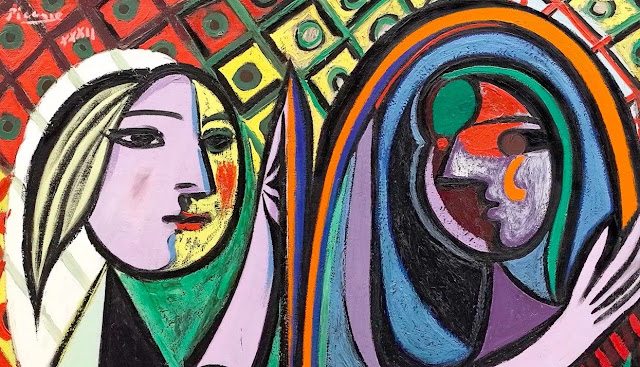
\includegraphics[width=0.8\textwidth]{img/picasso-1932}
\caption{\textsc{Pablo Picasso}. Fragmento de \emph{Joven mujer delante de un espejo}, 1932.  Óleo sobre lienzo, 162.3 x 130.2 cm. MOMA, Nueva York.}
\label{fig:picasso-1932}
\end{figure}

\section{Bitonalidad}
\label{sec:bitonalidad}

Hay una característica central en la obra musical de \textsc{Leguizamón}, indicada en alguna entrevista televisiva por el mismo autor: la presencia simultánea de dos imágenes sonoras conformando una única imagen compleja. La comparación con la pintura de \textsc{Pablo Picasso} es inevitable: una imagen compleja producto de la superposición de dos rostros, uno de frente y uno de perfil (ver Figura~\ref{fig:picasso-1932}).

Los acordes triadas fueron, durante mucho tiempo, la fundamentación del pensamiento armónico en la música occidental. Avanzado el siglo XIX, la creciente tendencia a utilizar acordes de más de tres notas no dejaba de hacer referencia a una única fundamental de cada uno de dichos acordes. Los llamados acordes \emph{errantes}\footnote{Un acorde errante ---tal es la denominación de \textsc{Arnold Schoenberg}--- es un acorde que es capaz de cumplir la misma función tonal en más de una tonalidad no-homónima. Típicos ejemplos de ellos son los acordes de séptima disminuida, los de quinta aumentada, los de sexta aumentada y los séptima dominante a distancia de semitono ascendente respecto a la tónica.}, aunque en sí poseen una única fundamental, sí pueden estar respondiendo a más de una tónica, por lo que su aparición en la escena musical es un importante antecedente para el surgimiento de la música politonal, es decir la música que tiene más de una tónica al mismo tiempo.

Otro antecedente histórico presente en la tonalidad que ayudó a desembocar en la bitonalidad está presente ya en el modo menor, cuando se enlaza el III grado con el \acorde.V..\sostenidotxt3..., enlace en el que la quinta del tercer grado ---en La menor, \emph{sol}--- se relaciona con la tercera del \acorde.V..\sostenidotxt3... ---\emph{sol\sostenidotxt}. La normativa tonal, justamente para evitar la presencia de dos tónicas simultáneas, prohíbe lo que se conoce como \emph{falsa relación}, obligando a introducir la tercera del \acorde.V..\sostenidotxt3... en la misma voz que la quinta del III grado produciendo así un ascenso cromática de la voz que impide la interpretación perceptual de la presencia de más de una tónica simultánea. Sin embargo, muy habitualmente en las prácticas populares la norma no se observa, apareciendo de facto la bitonalidad. El modo dórico, tan presente en algunas manifestaciones musicales folclóricas de Sudamérica que nutrieron al universo musical de Leguizamón, tiene en potencia la posibilidad de la bitonalidad, especialmente en la relación entre los grados VI y \acorde.IV..\sostenidotxt3..., donde la fundamental del primero y la tercera del segundo, de sucederse en voces diferentes, o de estar ésta en la línea melódica mientras el acompañamiento transcurre sobre el VI grado\footnote{Este fenómeno puede encontrarse en grupos folclóricos como \emph{Los Fronterizos}.}, la manifestación de la bitonalidad es ya un hecho.

\textsc{Ravel}, \textsc{Bartók} y \textsc{Stravinsky} son algunos de los exponentes europeos que explicitan en su obra la presencia de más de una tónica en la simultaneidad. \textsc{Villalobos}, \textsc{Revueltas} y \textsc{Ginastera} también lo hacen en América. \textsc{Leguizamón}, \textsc{Piazzolla} y \textsc{García}, más acá en el tiempo, incluyen en sus composiciones estas técnicas que ofrecen a los oyentes una complejidad armónica abordable por los oídos contemporáneos. Las resistencias y oposiciones que enfrentaron todos los compositores anteriormente citados, hoy ya han sido superadas, hoy ya encuentran en las percepciones de las mayorías eco favorable para esas sonoridades que fueran novedad durante el siglo pasado.

\section{Tonalidad y arquetipos}
\label{sec:tonalidad-arquetipos}

Dos son los arquetipos musicales rastreables en prácticamente todas las culturas humanas: la escala y el arpegio. Éste surge del despliegue en el tiempo de los cuatro primeros parciales de un sonido armónico\footnote{Un \emph{sonido armónico} es el que es susceptible de ser cantado, un sonido con altura determinada, un sonido que en su estructura de frecuencias conformantes existe una relación de múltiplos enteros de la frecuencia fundamental.}, mientras que aquélla es, en sus versiones ascendente y descendente, la garantía de un camino perceptualmente transitable a la vez que tranquilizante. Tanto una escala como un arpegio son fáciles de cantar para la inmensa mayoría de seres humanos, y si es fácil de cantar es porque es fácil de percibir.

\label{par:puente}Un \emph{puente de segundas}, en composición de melodías, es «esconder» una escala dentro de una melodía más compleja para que el oyente o el cantante tenga disponible ese arquetipo para su tranquilidad y facilidad de ejecución. Raro es el himno ---especialmente himnos nacionale--- que no posea en su línea melódica un puente de segundas. Podemos poner como ejemplo el himno ruso:

\begin{figure}[H]
\begin{ly}[ragged-right]
\relative {
  \key f \major
  \time 4/4
  \slurDashed
  a''2 ( g8 f e f
  g2 ) ( c,
  f ) ( e8 d c d
  e2 ) ( a,
  d4 ) ( c8. bes16 c4 ) f,
  f' e8. d16 c2
}
\end{ly}
\caption{Puente de segundas en los himnos del mundo: himno de Rusia.}
\label{fig:himno-ruso}
\end{figure}

Marcado con ligaduras punteadas, en la Figura~\ref{fig:himno-ruso} podemos observar el puente de segundas presente el el estribillo del himno de Rusia, conformando una escala descendente \musncp{\relative {a''2 g f e d c}} que dota a esta línea melódica tanto de belleza como de facilidad de entonación para muchas personas.

\begin{figure}[H]
\begin{ly}
\relative {
  \key f \major
  \time 2/4
  \partial 8
  c'8
  \slurDashed
  f4. ( f8
  f d e f
  g4 ) ( g8 f
  e4. c8
  a'4. ) ( a8
  a f g a
  bes4 ) bes8 a
  g4.
}
\end{ly}
\caption{Puente de segundas ascendentes en el himno de Leguizamón.}
\label{fig:segundas-ascendentes-himno}
\end{figure}

Observando esta característica de la tradición hímnica, Leguizamón construye la línea melódica del Himno a la Universidad Nacional de Salta sobre un puente de segundas ascendentes \musncp{\relative {\key f \major f'2 g a bes}} en la primera parte (ver Figura~\ref{fig:segundas-ascendentes-himno}) y otros dos puentes de segundas descendentes \musncp{\relative{\key f \major f''2 ( e d c\glissando ) a ( g f )}} en la segunda parte. El hecho de poseer dos puentes de segunda donde el primero empieza y termina en \nota{fa}{5} y \nota{do}{5} respectivamente, y el segundo empieza y termina en \nota{la}{4} y \nota{fa}{4} muestra al oyente y al intérprete, en forma aún más sutil que la escala, el arpegio de Fa mayor \hbox{\musncp{f''2 c'' a' f'},} representante de la tónica. Así, los dos arquetipos musicales presentes en toda cultura humana, presentes también están en la melodía del Himno a la UNSa de Leguizamón.

\begin{figure}[H]
\centering
\begin{ly}
\relative {
  \key f \major
  \time 2/4
  \partial 8
  c''8
  \slurDashed
  f4. ( f8
  f d e f
  \slurHalfDashed
  e4 ) ( c8 a
  c4. )
}
\end{ly}
\begin{ly}
\relative {
  \key f \major
  \time 2/4
  \partial 8
  \slurHalfDashed d''8 (
  bes4 ) bes
  bes4.
}
\end{ly}
\begin{ly}
\relative {
  \key f \major
  \time 2/4
  \partial 8
  \slurHalfDashed
  c''8 (
  a ) \slurDashed ( g a f
  g ) ( d e c
  f4. )
}
\end{ly}

\vspace{0.5cm}

\begin{ly}[notime]
\layout {
  \context {
    \Voice
    \consists Horizontal_bracket_engraver
  }
}
\relative {
  \key f \major
  <<{f''2\startGroup e d c\stopGroup s s} \\ {s2 s bes\startGroup a g f\stopGroup}>>
}
\end{ly}
\caption{Arpegio y escala en la melodía.}
\label{fig:arpegio-escala-cuchi}
\end{figure}

\noindent En rigor de verdad, \musncp{\relative{\key f \major f''2 ( e d c\glissando ) a ( g f )}} no es una fiel representación de la estructura melódica de los compases 26 al 34, sino el último Fragmento presentado en la Figura~\ref{fig:arpegio-escala-cuchi}, donde se puede ver una especie de solapamiento del desarrollo de dos puentes de segundas, uno desplegando el tetracordio superior \nota{fa}{5}-\nota{do}{5}, y otro cerrando el ciclo de la octava con el tetracordio inferior \nota{si\bemoltxt}{4}-\nota{fa}{4} de la tonalidad de la pieza. Ese solapamiento entre tetracordios se produce en los compases 30 y 31, visible en el segundo fragmento de la Figura~\ref{fig:arpegio-escala-cuchi}, compases éstos que presentan el verso \emph{hasta que al fin}, verso que rompe con la precedente simetría de 11 sílabas mostrado en el Cuadro~\ref{tab:ritmo-letra}. Aunque por un lado el solapamiento oscurece la presencia del arpegio, por otro ---y a pesar de estar en parte débil de tiempo--- el \nota{do}{5} en el \emph{levare} del compás 32 pasa a tener, en la percepción del oyente, un lugar jerarquizado por ser el inicio de un envión final que nos deposita en el último tramo de la pieza, y al ser esta nota perceptualmente importante, garantiza y aclara la presencia de la estructura arpegiada, la cual también está afianzada por la presencia del \nota{do}{5} del compás 29, en tiempo fuerte y con una duración de una \negrap que cierra la palabra \emph{ofrendarán}.

Aún no hemos llegado a la certeza estructural, ya que en la primera parte del descenso (compases 26 al 29, ver Figura~\ref{fig:arpegio-escala-cuchi}, primer fragmento) observamos una estructura \hbox{\musncp{\key f \major f''2 e'' c''},} no \musncp{\key f \major f''2 e'' d'' c''}, donde el \nota{re}{5} mencionado como estructural aparece en forma diferida y asociada a la relación de tercera descendente en los compases 30 y 31 con \emph{levare} transcripto en el segundo fragmento de la Figura~\ref{fig:arpegio-escala-cuchi}, y que completa juego con el tercer fragmento de la misma Figura con el descenso de tercera \musncp{c''2 a'}, conformando entre las tres partes una sucesión de terceras \musncp{\key f \major <e'' c''>2 <d'' bes'> <c'' a'>}, presentada parcialmente en el cuarto fragmento de la citada Figura, de carácter analítico, como solapamiento entre tetracordios. El no haber dicho en primer término lo de la sucesión de terceras y sí haber mencionado lo de la sucesión de tetracordios tiene que ver con que esta sucesión es estructuralmente más importante que la sucesión de terceras debido a que a partir del \emph{levare} del compás 34 hasta el final nos encontramos con una melodía cuya estructura responde, una vez más, a una demarcación de los inicios y finales de los tetracordios de la escala de Fa mayor \hbox{\musncp{\key f \major f'2 bes' c'' f''},} tal como muestra la Figura~\ref{fig:final-melo-estructura}.

\begin{figure}[H]
\begin{ly}
\relative {
  \key f \major
  \time 2/4
  \partial 8
  c'8
  \slurDashed
  f4. ( f8
  f d e f
  bes4. ) ( bes8
  bes g a bes
  c4 ) ( f8 g
  d4 e
  f2 ) \bar "|."
}
\end{ly}
\caption{Final de la melodía: estructura tetracordal.}
\label{fig:final-melo-estructura}
\end{figure}


La estructura melódica completa queda, pues, definida principalmente por notas que delimitan al tetracordio inferior puestas en forma ascendente y conectadas por un puente de segundas, seguidas por notas que delimitan el tetracordio superior conectadas por un \nota{mi}{5}, seguido por nuevamente el tetracordio inferior esta vez presentado en forma descendente como puente de segundas, para finalmente representar otra vez el tetracordio inferior, esta vez en un ascenso final y por salto directo entre el \grado{1} y \grado{4} grados (\emph{fa-si\bemoltxt}), finalizando con el tetracordio superior (\emph{do-fa}) haciendo oír sus notas extremas primero en forma directa (salto) y luego recorriendo el resto del tetracordio (\emph{re-mi-fa}).

\begin{figure}[H]
\begin{ly}[notime]
\layout {
  \context {
    \Voice
    \consists Horizontal_bracket_engraver
  }
}
\relative {
  \key f \major
  \hide Stem
  \slurHalfDashed
  f'2^"c.18"\startGroup g a bes\stopGroup \bar "||"
  f'^"c.26"\startGroup e4 ( c2\stopGroup ) \bar "||"
  d4^"c.30" ( bes2\startGroup ) c4 ( a2 ) g f\stopGroup ~\bar "||"
  f2^"c.34"\startGroup bes\stopGroup
  \slurHalfSolid
  c^"c.38"\startGroup ( f4 ) d2 e f\stopGroup \bar "|."
}
\end{ly}
\caption{Estructura de la melodía.}
\label{fig:estructura-melodia}
\end{figure}

Además de haber hecho presente los arquetipos de escala y arpegio, como acabamos de ver, hace el autor aparecer un tercer arquetipo: el de dividir la octava en dos partes iguales, dos cuartas justas conteniendo cada una de ellas cuatro sonidos es decir un \emph{tetracordio}. Innumerables y de diversas culturas son los ejemplos ancestrales de uso de estructuración de melodíos en esta forma, usando como puntos de apoyo de las frases musicales a las notas de partida y llegada de cada uno de los tetracordios en los que se secciona la octava, base de toda música tonal. Desde cantos antifonales y responsoriales donde grupos antagónicos o complementario, o un líder y sus seguidores cantan alternativamente unos en las notas de un tetracordio y los otros responden sobre las notas del otro tetracordio. Esa genética cultura, además de los dos arquetipos universales, es la que se encuentra inscripta en la melodía del Himno a la Universidad de Salta de Gustavo Leguizamón.


\section{Tonalidad de tonalidades}
\label{sec:tonalidad-tonalidades}

Desde el alto barroco hay conciencia en los compositores acerca de una tonalidad que contiene a otras tonalidades. El sistema tonal es la síntesis de los doce modos eclesiásticos\footnote{La teoría musical de la Edad Media definió un total de siete modos, \emph{dórico, frigio, lidio, mixolidio, eólico, jónico y locrio}, a los que denominó \emph{modos auténticos}, y derivó de ellos siete más, los llamados \emph{modos plagales}. De esos catorce modos eliminó dos (locrio e hipolocrio) por considerarlos no aptos para la práctica musical.} resumidos en las modos mayor y menor. Al ser siete los grados armónicos (acordes) de una tonalidad, donde tres son mayores, tres menores y uno disminuido, se observó y no se desaprovechó la oportunidad de interpretar a cada grado mayor o menor como tonalidades enteras dentro de la tonalidad, cada una con sus propios grados armónicos. El VII grado del modo mayor y el II del modo menor sufrió, en este sentido, el mismo destino que en su momento sufriera ---y por motivos similares--- el modo locrio: la ignorancia, la periferia desde la cual luego montaría éste su revolución\footnote{El VII grado del modo mayor y el II del modo menor contienen el intervalo más complejo de percibir, el \emph{tritono}, el cual desempeñó y desempeña un papel central en el desarrollo de la composición músical}. Al ser la tonalidad un sistema jerarquizado, donde cada nota cumple función y cada conjunto de estandarizado de notas (acordes) cumple función en un escenario donde se libra una lucha por el poder, por el privilegiado lugar de la tónica, a la vez los grados armónicos subordinados a cada grado de la tonalidad cumplirán, en el contexto general, la misma función que su «jefe regional» cumple en la tonalidad principal. Por ejemplo, aunque un II grado, en general cumple una función de \emph{subdominante}, el II grado de un V grado (II/V) cumple, en la tonalidad principal, la función que cumple el V grado, es decir función de \emph{dominante}, o, dicho de otra manera, «donde manda capitán no manda marinero».

Esta noción de \emph{metatonalidad}, de tonalidad de tonalidades, en la práctica musical folclórica se ve acotada casi exclusivamente a la presencia de \emph{dominantes secundarias}, es decir a utilizar el V grado de cada grado de la escala. Usar otro grado que no sea el V/x es, en la música popular de medio siglo atrás un inequívoco síntoma de arte evolucionado y con un grado de complejidad a la que afortunadamente la sociedad argentina está acostumbrada por poseer una notable riqueza en sus músicas de consumo masivo. Volvemos acá a mencionar a Piazzolla, podemos agregar a Mariano Mores, y saludar nuevamente a Charly García como pares de Leguizamón en cuanto compositores que presentan a su público una elaboración armónica que no subestima al oyente.

El compás 16 del \emph{Himno} ya nos presenta un acorde \musncp[voffset=-4pt]{\key f \major \clef alto <d c' es' fis' a' c''>2},ajeno éste al diatonimso de Fa mayor. Por ello, para hallar el significado armónico de tal acorde nos conviene bucear en alguna de las regiones, de los grados de Fa mayor. En este caso, notamos que la estructura del acorde corresponde a una dominante, pero dominante de qué grado es la pregunta que debemos hacernos, V grado de qué grado, y al ser \emph{re} la fundamental de dicho acorde, sale a la luz que es V/II, es decir dominante de la relativa menor de la subdominante (D/rS), con novena y séptima menores, por lo que su cifrado es \acorde.V..\bemoltxt9.7.\sostenidotxt3./II. Hasta acá, nada fuera de libreto respecto a los usas habituales en la música popular. Sin embargo, lo notorio surge de inmediato, al resolverse este acorde no donde se espera, es decir en el II grado de Fa, sino ¡sobre el V grado de Fa! Es muy habitual, en una música que renuncia a lo revolucionario en favor de la transformación ---y la de Leguizamón lo es--- proceder modificando el camino que pasa por tres puntos \emph{a, b, c} a un camino que da por obvio al punto \emph{b} pasando directamente de \emph{a} a \emph{c}. Así, cuando se espera la semicadencia V/II - II - V al final de la introducción del \emph{Himno}, nos encontramos con el enlace directo V/II - V, del punto \emph{a} al punto \emph{c} sin escala intermedia. Suena novedoso, pero no revolucionario; transforma, innova al tiempo que no deja a los oyentes en un terreno ni hostil ni completamente desconocido, pero no desprovisto de sorpresa.

El mismo acorde es oído con anterioridad, en el compás 8, también en la introducción de la pieza, pero en esta ocasión el acorde no se dirige hacia la dominante, sino que cumple la función formal de suspender la semifrase antes de retomar la segunda semifrase, la cual parte de tónica. Si el camino \emph{a - b - c}, es resumido en \emph{a - c} en los compases 16 y 17, en los compases 8 y 9 se resume a la presencia del único punto inicial del camino, el punto \emph{a}, el acorde \acorde.V..\bemoltxt9.7.\sostenidotxt3./II, sin resolución alguna, suspendiendo, dejando abierta la semifrase inicial de la introducción del himno.

Tanto en su aparición en compás 8 como en la de compás 16, el V/II está presente bajo el fragmento melódico \mus{\key f \major \time 2/4 c''4 ~ \tuplet 3/2 {c''8 a' bes'} c''4_"V/II"}. La diferencia formal y consecuentemente funcional está dada por el nada irrelevante hecho de la repetición del fragmento melódico  en compás 16 con \emph{levare}, siendo \mus{\key f \major \time 2/4 \partial 4 \tuplet 3/2 {r8 a' bes'} c''4_"V/II" ~ \tuplet 3/2 {c''8 a' bes'} c''4_"V"} una cadencia evitada sobre el V grado que convierte al V/II en un acorde con función subdominante que precede justamente al V, mientras que en compás 8, al no estar repetido el motivo melódico, el mismo acorde V/II cumple sorpresivamente la función de \emph{dominante}, ya que la ausencia del V con posterioridad al V/II, lo hace indirectamente representante de la dominante, aunque tal acorde surja de la región de la relativa de la subdominante.

\section{Funciones armónicas y bitonalidad}
\label{sec:funciones-bitonalidad}

Para finalizar este breve análisis del \emph{Himno} en sus aspectos armónicos sobresalientes, ponemos el foco en los compases del 27 al 29:

\begin{figure}[H]
\centering
\begin{ly}
manoderecha = \relative {
  \clef treble
  \key f \major
  \time 2/4
  \set Score.currentBarNumber = #27
  \bar ""
  <b' f'>8 d <b e> f'
  <f, e'>4 <g c>8 <e a>
  <es fis c'>4. d'8

}
manoizquierda = \relative {
  \clef bass
  \key f \major
  \time 2/4
  b,8 gis' d'4
  <f,, c' a'>2
  <d' c'>
}

\score {
  \new PianoStaff <<
    \new Staff \manoderecha
    \new Staff \manoizquierda
  >>
}
\end{ly}
\caption{Dominante del III grado resolviendo en I.}
\label{fig:V-III}
\end{figure}

El acorde que encontramos en el compás 27 es el \acorde.V.\becuadrotxt5.9.7.\sostenidotxt3./III, acorde que convencionalmente resuelve sobre su «jefe» regional, el III grado. Sin embargo, en compás 28, en lugar de ese esperado III nos topamos de frente con el \acorde.I..9.7.., el cual, en compás 29, resuelve sobre el ya mencionado, en sección~\ref{sec:tonalidad-tonalidades}, \acorde.V..\bemoltxt9.7.\sostenidotxt3./II, cumpliendo él, una vez más, la función de semicadencia ---esta vez dejando abierta la expectativa de resolución sobre el II grado que, esta vez, sí se cumple en compás 30, inicio de una nueva frase y un nuevo verso. ¿Cómo se explica que el \acorde.V.\becuadrotxt5.9.7.\sostenidotxt3./III resuelva en \acorde.I..9.7..? Si observamos, en la Figura~\ref{fig:V-III}, la mano derecha del compás 28, notaremos que la sensible descendente \nota{fa}{5} del compás anterior presente en la melodía resuelve sobre el \nota{mi}{5}, séptima del I grado, siguiendo la línea melódica con el despliegue del arpegio de La menor, apoyado por el \emph{voicing} que presenta, bajo el \emph{do} a la novena del I y bajo el \emph{la} la séptima del mismo grado, pero que a la vez son la séptima y la quinta del acorde de La menor. ¿Estamos ante una «pincelada» de bitonalidad, donde conviven los centros tonales de \emph{fa} y \emph{la}? Nuestra respuesta: sí. El \acorde.V.\becuadrotxt5.9.7.\sostenidotxt3./III sí está resolviendo sobre un \acorde.III.6.7..., que al tener en el bajo el \nota{fa}{2} (mano izquierda) produce un acorde complejo que, sin profundizar, tendemos a reconocer como un acorde \acorde.Fa..9.7.. y no como un \acorde.La.Fa.7.... En definitiva, en este pasaje del \emph{Himno}, como en tantos otros pasajes de la obra musical de Leguizamón, tenemos, al mismo tiempo, un rostro de frente (\emph{fa}) y de perfil(\emph{la}), como si de una pintura de Picasso se tratara.
